% \section{Higher Order Probabilistic Inference}

% People often entertain beliefs about probability statements.
% For instance most people accept even expert-given odds that a particular sports team will win a tournament, or politician will win an election, with a degree of scepticism.
% % and therefore (iii) perhaps we need a new or extended theory of probability to be able to reason about these facts.
% The apparent failure of probabilistic expressions to distinguish between these cases led to alternative formalisms of uncertainty \cite{Shampher}, but within the probabilistic framework both Pearl \cite{} and HyBerg{} demonstrated that such higher order distributions were induced from the original model, no new machinery was needed.
% Many scenarios require the ability to both define and condition probability distributions over either random variables or properties of random variables (e.g. expectations).
% In this section we introduce the random conditional distribution ($\randcond$) to support this task.
% $\rcd$ is best explained through example:


% % Higher order probabilities emerge whenever there is a distinction between subjective and objective probabilities.
% % For example many systems which verify probabilistic statements make assertions such as this assertion holds with a probability greater than 0.9.
% % This distinction between the objective probability with which the assertion holds and the bound that can be proved reflects the gap in the reasoning capacity of the agent.

% % Further still, higher order distributions is a more general concept that higher order probabilities, encompassing it as a special case.
% % Consider an assertion about the fairness of a hiring program $P$ that takes as input a vector of arguments $v$ representing a job applicant’s record and returns a Boolean value indicating whether the applicant is hired.
% % One of the arguments $v$ 


% Consider a coin toss in the basement of a unscrupulous gambler, and having the belief that the coin could be fair or be biased towards tails, but also that the coin-tosser may bias its outcome through sleight of hand.

% \begin{figure}[!htb]
% \centering
% 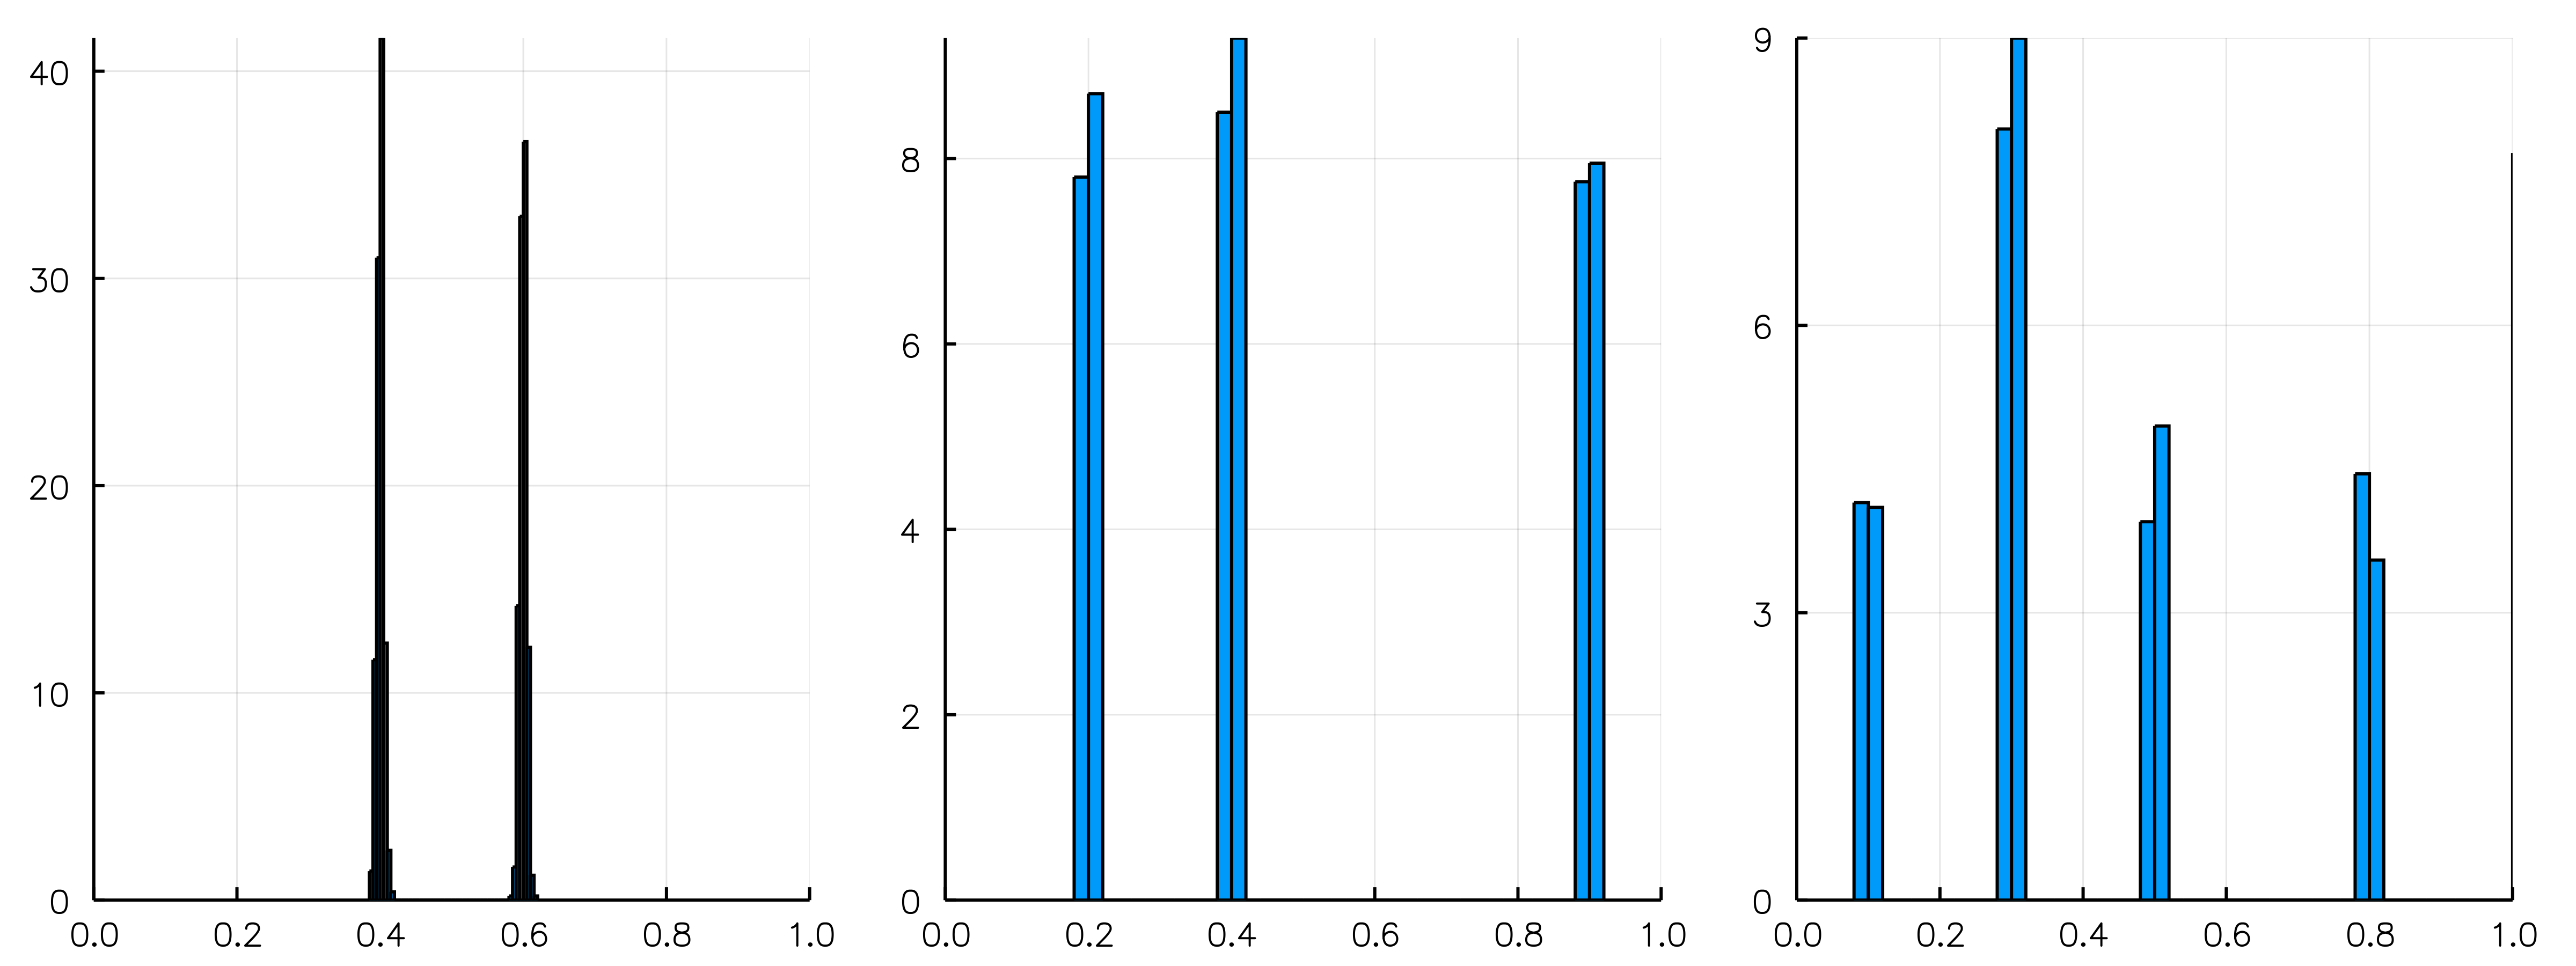
\includegraphics[width=0.9\linewidth]{figures/rcd}
% \caption{Imagine observing the outcome of flips of a coin of unknown fairness, e.g., $coin = \bern(w + b)$ comes up heads with probability $W + b$, where weight $w = \unif(\{-0.2, 0, 0.2\})$ is uniformly distributed,  $b = \unif(\{-0.2, 0, 0.5\})$
% The marginal probability that the $P(coin = H) = 0.5$ is equal to that of a bank-minted, fairly-tossed coin.
% Put another way, despite the fact that a gamblers coin tossed by untrustworthy tosser and a freshly minted coin have the same overall probability of turning up heads, we would not be very surprised if the fraction of heads appearing in a large number of the gambler coin tosses deviated greatly from 0.5, but very surprised if it occurred with bank coin tosses.
% The random conditional distribution allows us -- among other things -- to induce distributions over probabilities directly from the original model, distinguishing these two scenarios.
% \ref{rcd} demonstrates .  From left to right random samples from (a) $\mean{\rcd(coin, fair)}$, (b) $\mean{\rcd(coin, b)}$ (c) $\mean{\rcd(coin)}$}
% \label{fig:rcd}
% \end{figure}

% TODO: Higher order more general that reasoning over beliefs





% \subsection*{Lifting}
% Lifting is a process which gives meaning to expressions such as $X+X$ when $X$ is a random variable rather than a number.
% To lift a function (such as $+$) means to It constructs a functional defined on $T$-valued random variables from a function defined on values of type $T$, mechanising the principle that a transformation of a random variable yields a random variable.
% Lifting is important because syntactically, it is more convenient to use random variables as if they were values rather than compose functions in measure theoretic notation.
% In addition, it allows us to repurpose existing programs expressed in values of type $T$ (e.g., ray-tracers which take geometric objects as input) to $T$-valued random variables (distributions over objects), without modification.

% To treat random variables as values we interpret operations on them \emph{pointwise}.
% % Given a function $f$ with domain $T$, we lift it to the domain of a random variable of codomain $T$.
% Let $X:\Omega \to T_1$ be a random variable, and $f:T_1 \to T_2$ be a function, then $Y = f(X)$ is a random variable defined as:
% $$
% Y(\omega) = f(X(\omega))
% $$
% Lifting extends to multivariate functions in the obvious way, e.g.:
% $$
% X + X = \omega \mapsto X(\omega) + X(\omega)
% $$
% More generally lifting is performed through an operator $\lift$:
% \begin{definition}
% Let $f: T_i \times \cdots \times T_n$ be an $n$-ary multivariate function, and denote by $e_\omega()$ the evaluation functional defined by $e(X, \omega) = x(\omega)$ if $X$ is a random variable and $e(X, \omega) = X$ otherwise.
% $\lifted{f}: (\omega \to T_1) \times \cdots \times (\omega \to T_n)$ where $f(X)$
% \end{definition}

% \improvement{WHY is lifting defined pointwise}

% \subsection*{Conditional Random Variable}
% Probabilistic inference is achieved through conditioning.
% To condition means to restrict the universe to only those scenarios where a condition holds.
% A predicate $Y: \Omega \to \{0,1\}$ can be used to restrict a probabilistic model to a subset of the uncertainty.
% That is, every event $A$ has a characteristic predicate $Y$ defined by
% $Y(\omega) = 1$ if $\omega \in A$, otherwise $Y(\omega) = 0$.
% Equivalently, the image of $A$ under $Y$ is $\{1\}$ and the preimage of $\{1\}$ under $Y$ is $A$ is 
% $Y^{-1}(\{1\}) = \{ \omega \in \Omega : Y(\omega)\} = A$

% The primary mechanism for conditioning is $\cond$, which constructs conditional random variables:
% \begin{definition}
% Let $X:\Omega \to T$ be a random variable, $Y$ an indicator function, and $X_{|Y}: \Omega_{|Y} \to T$ defined as $\cond(X, Y)$ be a conditional random variable defined as: $X_{|Y}(\omega) = X(\omega)$.
% $X_{|Y}$ is defined on a conditioned probability space $(\Omega, \Sigma, \mu_{|Y})$ where $\mu_{|Y}$ is a conditional measure: $
% \mu_{|Y}(A) = \mu(A \cup Y^{-1}(\{1\})) / \mu(Y^{-1}(\{1\})$.
% That is, $\cond: (\Omega \to T) \times (\Omega \to \{0, 1\}) \to (\Omega \to T)$ is a operator that restricts the domain of $X$ to those inputs consistent with $Y$.
% \end{definition}

% Conditional random variables.  Operations on conditional random variables constructs further conditional random variables.
% Observe that if two conditional random variables are composed then:

% $$
% \begin{aligned}
% (f(X_{|Y}))(\omega)&=f(X_{|Y}(\omega))&{\text{ where } Y(\omega)}\\
% (f(X_{|Y_1}, X_{|Y_2}))(\omega)&=f(X_{|Y}(\omega))&{\text{ where } Y_1(\omega)} \wedge Y_2(\omega)\\
% % (\lambda f)(x)&=\lambda \cdot f(x)&{\text{(pointwise multiplication by a scalar)}}
% \end{aligned}
% $$

\section{The Random Conditional Distribution}
The random conditional distribution of $X$ given $\Theta$ -- which we denote $\rcd(X, \Theta)$ or $\rcdxy{X}{\Theta}$ -- is a random distribution: a random variable which takes values in the domain of random variables.
Informally, $\rcdxy{X}{\Theta}$ is a probability distribution over random variables of the same type as $X$, where each random variable in that distribution corresponds to an element of $\theta \in \Theta$ and is weighted by the prior probability of $\theta$.
Formally, $\rcd$ is a distribution over conditional random variables:

% The primary mechanism for conditioning is $\cond$, which constructs conditional random variables:
\begin{definition}
Let $X:\Omega \to T$ be a random variable, $Y$ an indicator function, and $\conds{X}{Y}: \Omega_{|Y} \to T$ be a conditional random variable defined as: $X_{|Y}(\omega) = X(\omega)$.
$X_{|Y}$ is defined on a conditioned probability space $(\Omega, \Sigma, \mu_{|Y})$ where $\mu_{|Y}$ is a conditional measure: $
\mu_{|Y}(A) = \mu(A \cup Y^{-1}(\{1\})) / \mu(Y^{-1}(\{1\})$.
% That is, $\cond: (\Omega \to T) \times (\Omega \to \{0, 1\}) \to (\Omega \to T)$ is a operator that restricts the domain of $X$ to those inputs consistent with $Y$.
\end{definition}


\begin{definition}The random conditional distribution of a random variable $X: \Omega \to T_1$ given $\Theta: \Omega \to T_2$ is a random variable $\rcdxy{X}{\Theta}: \Omega \to (\Omega \to T_1)$, defined as:
\begin{equation}\label{eq:rcd}
(\rcdxy{X}{\Theta})(\omega) = \conds{X}{\Theta = \Theta(\omega)}
\end{equation}
\end{definition}
For example if $\Theta = \bern(0.4)$ and $X = \normal(\Theta, 1)$, then $\rcdxy{X}{\Theta}$ is a random distribution comprised of two normal distributions $X_1 = \conds{\normal(\Theta, 1)}{\Theta = 1}$ and $X_2$.
The probabilities of $X_1$ and $X_2$ with respect $\rcdxy{X}{\Theta}$ are determined by the prior probabilities of the different outcomes of $\Theta$: $P((\rcdxy{X}{\Theta}) = X_1) = 0.4$ and $P((\rcdxy{X}{\Theta}) = X_2) = 0.6$.

A random conditional distribution is most useful when used in combination with other functions.
Expectation is perhaps the most important example, which when composed with $\rcd$ produces conditional expectation.
Expectation $E : (\Omega \to \mathbb{R}) \to \mathbb{R}$ is a functional that maps a random variable to a real value.
When $X$ is a real valued random variable, $\rcdxy{X}{\Theta}$ is not real valued, and hence not a valid argument to $E$.
However, just as arithmetic operations such as $+$ and $-$ extend from the domain of numbers to the domain of random variable (pointwise	 $X + Y = \omega \mapsto X(\omega) + Y(\omega)$), $E$ extends from the domain of random variables to the domain of random variables over random variables in precisely the same way.
% Since random variables are themselves functions, $E$ is an operator, functional or more generally a higher-order function.  
% As described in section X a function with domain $T$ can be lifted to a functional of $T$-valued random variables.
% $T$ is purposefully left abstract, because in addition to lifting functions defined on the reals etc, we can lift functions defined on random variables.
% Expectation is a cannonical example of a random variable valued function, with type $E : (\Omega \to \mathbb{R}) \to \mathbb{R}$.
That is, $\ee$ has a lifted counterpart $\lifted{\ee} = \lift(\ee)$ with type $\lifted{\ee} : (\Omega \to (\Omega \to \mathbb{R})) \to (\Omega \to \mathbb{R})$, which maps a distribution over real valued random variables to a distribution over real values (expectations).
$$
\lifted{\ee}(X)(\omega) = \mean{X(\omega)}
$$
$\rcd$ composed with $\ee$ constructs conditional expectation (with respect to a random variable $\Theta$):
\begin{equation}
\lmean{\rcdxy{X}{\Theta}} = \lmean{\omega \mapsto \conds{X}{\Theta = \Theta(\omega)}} 
                    = \omega \mapsto \mean{\conds{X}{\Theta = \Theta(\omega)}}\\
\end{equation}
The final term $\omega \mapsto \mean{\conds{X}{\Theta = \Theta(\omega)}}$ is the definition of a conditional expectation with respect to a random variable $\mean{(X\mid \sigma (Y))(\omega)} = \mean{X \mid Y = Y(\omega))}$.

% Move to appendix?
% Equation \ref{eq:rcd} is a construcive definition of $\rcd$; here we define it declaratively:
% Let $\mu_\Theta = \mu \circ \Theta^{-1}$ denote the push forward measure of		 $\mu$ with respect to $\Theta$, $\tilde{X} = \randcond(X, \Theta)$, and $X^* \subset \tilde{X}$ be a set of random variables, then:
% $$
% \mu_{\tilde{X}}(X^*) = \mu_\Theta(\varphi^{-1}(X^*))
% $$

\improvement{This needs to be made clearer. Will there be issues taking measures in function space?}

\improvement{Need to define space of functions that measures exist on. Then define curry(X, $\Theta$), random variable on functions, to take measure given by pullback to $\Theta$ }

\improvement{Define: RCD of one argument $\rcd(X)$}

% \subsection{Higher Order Graphical Model}

% Probabilistic inference means to construct and condition random variables.
% In measure theory, a random variable is a function from a sample space $\Omega$ to $T$, where $T$ could for example be $\mathbb{R}$, but any type in general.
% $\Omega$ is understood as the universe of possible scenarios that could occur, or in sampling terms, as the random inputs to a random variable.
% Measure theory formalizes uncertainty by assigning probabilities to sets of possible scenarios, called events.
% The measure of an event represents a degree of belief that the event could occur, and is determined by a probability measure $\mu:\Sigma \rightarrow [0,1]$ where $\Sigma$ is a sigma-algebra (measurable subsets of $\Omega$).
% An event $A$ is impossible if $\mu(A)=0$, and certain if $\mu(A)=1$.

% We formulate $\rcd$ with respect to a form of directed graphical model.
% Higher order directed graphics are similar to standard bayesian networks but depart from them in two significant ways.
% First, the semantics of a graph is defined in terms of measure theoretic random variables, in contrast to probability mass or density functions, which means that every node is a deterministic transformation and all randomness is considered external to the system.
% Second this graph formalism is based on measure theoretic probability.

% \begin{definition}
% A higher order Bayesian Network $\mathcal{G}(V,E)$ is a directed acyclic graph, where $V$ are the nodes and $E$ are the edges of the graph.
% Nodes correspond to random variables, measurable functions from a sample space $\Omega$ to some output type $T$.
% Let $V_{\omega} \subseteq V$ denote the subset of variables without parents.
% Higher order graph are able to express both functions between  variables and functions of variables.
% Standard (non higher order) models are expressed using edges in $E_\circ$ (read $E$ compose).
% A composition edge from $A$ to $B$ denotes that $B$ functionally (and causally) depends on $A$.
% More precisely $A \to B$ denotes the composition $B \circ A$.
% Since $A$ is random variable, this composition is a random variable $\omega \mapsto B(A(\omega))$.
% \end{definition}
% Application edges in $E_{apply}$ denote function application.
% If a node $A$ is at the source of a directed edge in $E_{apply}$ it is taken as a value to be given as input to the node at the tail.
% % Let $f : V \to what$ map each node to a corresponding function, and $id : V_{\omega} \to \mathbb{N}$ map each parent-free node to a unique integer.
  
% \begin{align*}
% \mu &= \mathcal{N}(0, 1) \\
% X &= \mathcal{N}(\mu, 1) \\
% \tilde{X} &= \mathbb{E}(\rcdxy{X}{Y})
% \end{align*}


% \subsection{Efficient Construction of the Random Conditional Distributions}

Each outcome of a random conditional distribution is a conditional random variable which, in the general setting, can be a challenge to sample from.
In this section we demonstrate how to efficiently construct the random conditional distribution in a wide class of scenarios.

Recall that $(\rcdxy{X}{\Theta})(\omega) = \conds{X}{\Theta = \Theta(\omega)}$.
A realization $\conds{X}{\Theta = \Theta_c}$ of $\rcdxy{X}{\Theta}$ is a conditional random variable which may be difficult to sample from.
Instead, under modest conditions (theorem \ref{thm:path}) it is permissible to use a different distribution which is easier to construct:  $\ridxy{X}{\Theta}$ which \emph{fixes} rather than conditions $\Theta$:
\begin{equation}\label{eq:rid}
(\ridxy{X}{\Theta})(\omega) = \conds{X}{\Theta^a = \Theta^a(\omega) \text{ for all } \Theta^a \in \{ \Theta \} \cup \text{ancestors of } \Theta}
\end{equation} 
$\rcdxy{X}{\Theta}$ is distinct from $\ridxy{X}{\Theta}$ because in the former the parents of $\Theta$ are not fixed and hence for some realization $\conds{X}{\Theta = \Theta_c}$ we must consider all the possible scenarios which would result in $\Theta = \Theta_c$.
In contrast, 
$\ridxy{X}{\Theta}$ is always efficient to construct:

\begin{algorithm} 
\end{algorithm}

It is permissible to use $\ridxy{X}{\Theta}$ as a substitute for $\rcdxy{X}{\Theta}$ when they are equivalent, which is not always the case, consider:
\begin{align*}
\alpha &= \rade(0.5) \\
\beta &= \bern(0.5) * \alpha \\
\gamma &= \bern(0.5) + \alpha + \beta
\end{align*}

Random conditional distributions (such as $\rcdxy{\gamma}{\beta}$) can be induced from this model which are not equal to the corresponding "fixed" random conditional distribution: $\ridxy{\gamma}{\beta}$.
For example the distribution over expectations $\lmean{\rcdxy{\gamma}{\beta}}$ and $\lmean{\ridxy{\gamma}{\beta}}$ do not even have the same support.
However in other scenarions they are the same, e.g. $\rcdxy{\gamma}{\alpha} = \ridxy{\gamma}{\alpha}$.

Verifying equivalence of two random variables (let alone two random distributions) is undecidable in theory \ref{} and intractable in practice, putting us at risk of swapping one hard problem for a harder one.
Fortunately, the causal structure of the model provides sufficient (but not neccesary)ee conditions to determine if $\ridxy{X}{\Theta} = \rcdxy{X}{\Theta}$:
% Intuitively, the first result can be substitued because it sucks, while the seon dosn't suck.

\todo{Maybe use d-separation. $\Theta$ d-separates $X$ from its ancestors}
\begin{theorem} $\rcdxy{X}{\Theta} = \ridxy{X}{\Theta}$ when all paths from the ancestors $\Theta$ to $X$ pass through $\Theta$
\end{theorem}
\begin{proof}
To prove this theorem, it is crucial to formalize the structural assumption. The ancestors of $\Theta$ have no path to $X$ that doesn't pass through $\Theta$. This means that conditioned on $\Theta$, any ancestor of $\Theta$, $\Theta^a$, is independent from $X$, i.e.
\begin{equation*}
\conds{X}{\Theta, \Theta^a} = \conds{X}{\Theta} \quad \text{for all } \Theta^a \in \text{ancestors of } \Theta
\end{equation*}
Therefore, using \eqref{eq:rid} we obtain the following identity for all $\omega$
\begin{equation*}
(\ridxy{X}{\Theta})(\omega) = (\conds{X}{\Theta = \Theta(\omega), \Theta^a = \Theta^a(\omega) \text{ for all } \Theta^a \in \text{ancestors of } \Theta}) = \conds{X}{\Theta = \Theta(\omega)}
\end{equation*}
which concludes the proof that $\rcdxy{X}{\Theta} = \ridxy{X}{\Theta}$.
\end{proof}

% For example, to construct a set of samples from $\mean{\rcdxy{X}{Y}}$, we could:
% \begin{itemize}
% \item Unconditionally sample $Y$ to yield $y_c$.
% \item Sample $X^*$ from $\tilde{X}$ such that $X^* = X \mid Y = y_c$, where $y_c = Y(\omega_c)$ is a realization of $Y$
% \item Find $\Omega^* \subset \Omega$ such that $Y(\omega^* \in \Omega^*) = y$
% \item Compute $\mean{X^*}$ with respect to $\Omega^*$
% \end{itemize}

% Step 2 is hard for all the same reasons that conditioning is hard in general.
% However, we can exploit the fact that the condition $Y = Y(\omega)$ in $\rcdxy{X}{Y}$ is not an arbitrary condition, in effect, it is conditioning on the prior.

% \begin{itemize}
%   \item Unconditionally sample $Y$ to yield $y_c$, cache its input $\omega_c$ (i.e., $Y(\omega_c) = y_c$)
%   \item Compute $\mean{X}$ 
% \end{itemize}

% This sequence is identical in distribution to the first sequence, but dramatically easier to compute.